\subsection{Scenarios}
\label{subsect:Scenarios}
	\subsubsection{Scenario 1}
		Oscar is a businessman who travels a lot and he would like to organize his travels quickly and precisely. A friend advises him to try Travlendar+. Oscar enters the Travlendar+ website and loads the registration page by clicking on the 'signup' button, he fills all the mandatory fields and then he receives a confirmation email and he clicks on the confirmation link inside.
Then Oscar log in and starts using Travlendar+.
	\subsubsection{Scenario 2}
		Nigel lives in Milan and tomorrow he’s going to have an appointment in Lecco, so he has to decide how to reach his appointment location; Nigel accesses the log in page from his personal computer's browser, fills the username and password fields and click on the 'confirm' button and after he clicks on the dedicated button to add a new event, he fills all the requested fields, including setting the events type as 'work meeting' in order to obtain a proper suggested travel means according to the situation and confirms the event creation. The day after Nigel travel to lecco according to the travel schedule proposed by his Travlendar+ app, reaching in time his appointment.

	\subsubsection{Scenario 3}
		Jasper insert an event into his Travlendar+ calendar but the location of his event is too far away his previous event and doesn't exist a feasible path to reach the event’s location in the allotted time. Jasper is notified by a warning that he will not be able to reach his appointment in time.	
	\subsubsection{Scenario 4}
		Ophelia insert a new event into his Travlendar+ calendar but that events overlaps with another already existing event. Ophelia is notified by her app and the system asks Ophelia to choose which one of the overlapped event she wants to attend, she choose the event she has just inserted. She reads then the travel means proposed to respect hers new time schedule.
	\subsubsection{Scenario 5}
		Henrietta wants to personalize hers Travlendar+ experience, so she on the ‘menu’ button and then the preferences ‘button’. She select her preferred travel means, she choose to obtain always the fastest path and then, since she walks with a limp, she insert a maximum walking distance of 500 m. Before clicking on the confirm button she see a polluting trucks outside hers window and then she decide to follow always travel paths that minimize carbon footprint. She selects the relative option in hers preferences. She clicks on the ‘confirm’ button and she observe that her suggested travels are changed according to her preferences.
	\subsubsection{Scenario 6}
		Arthur can’t concentrate on his work if he doesn't eat his lunch between 12.00 and 13.00 and he need at least 25 minutes to consume a proper lunch.
So Arthur inserts a flexible break event into his Travlendar+ calendar in order to be sure that every day his app reserve a time slot for lunch every day.
After a week Arthur inserts a new event whose travel overlap with his flexible lunch event and his app notifies him. Arthur decide to ignore the warning, since he'll eat during his travel.
	\subsubsection{Scenario 7}
		Gwendolyn looks at her Travlendar+ app and discover that the next day she has to travel first by train to Milan and then take a bike of MoBike’s sharing system in Milan. She clicks on the train travel slot in order to buy the proper ticket and the apps redirect her in the right Trenord’s online shop webpage. When she is about to buy the ticket she suddenly remember that she has a weekly Trenord pass, so she cancel the transaction and add her pass informations into her Travlendar+ app in order to do not make the same mistake twice. The next day Gwendolyn take the train to Milan and when she arrive she opens her Travlendar+ app in order to find the nearest bike of MoBike’s. Gwendoline arrives in time at her appointment.
	\subsubsection{Scenario 8}
		Harvey have to reach an appointment near his home next week and then he adds an event in his Travlendar+ calendar. He observe that the suggested travel means is using a bike. The day before his appointment the weather forecast rain and so Harvey is notified by his app that due to the forecast he should avoid to take the bike, suggesting instead to reach his appointment by car.
	\subsubsection{Scenario 9}
		Sara inserts an event in her Travlendar+ calendar, and she looks at the proposed travel path. Since she didn't like the proposed travel she clicks on the proposed path and select another feasible alternative. The next day Sara will travel according to the travel path she likes more.	
	
\subsection{Use case descriptions}
\label{subsect:Use case descriptions}

	\subsubsection{Registration}
		\begin{table}[H]
	\begin{center}
		\begin{tabular}{ | p{0.3\textwidth} | p{0.7\textwidth} | }
		\hline
		Participating actors & Generic visitor\\
		\hline
		Entry Condition & There are no entry conditions.\\
		\hline
		Event Flow & 
			\begin{enumerate}
				\item The visitor clicks on the “Register” button displayed onto the homepage;
				\item The visitor fills all the mandatory fields shown required by the system including his email, his password (twice) and a captcha;
				\item The visitor clicks on “Confirm” button;
				\item The visitor receives a confirmation email and clicks on the confirmation link;
				\item The system saves all user data inserted.
			\end{enumerate} \\
		\hline
		Exit Condition & The visitor’s registration is completed successfully, so the visitor is registered as an user of Travlendar+ and he can log in into the system as a registered user. \\
		\hline
		Exception & If:
				\begin{itemize}
   					\item The visitor insert an email already connected to an existing account;
   					\item Insert invalid infos into in some mandatory field;
   					\item Leave empty a mandatory field;
   				\end{itemize}
   		Then the system will request the visitor to complete/ revise all uncorrected field, highlighting them.
if the visitor doesn’t activate the account, after a month the activation link will expire and all user data will be deleted.\\ 
		\hline
		\end{tabular}
	\end{center}
	\caption{registration use-case}
\end{table}
		
	\subsubsection{Login}
		\begin{table}[H]
	\begin{center}
		\begin{tabular}{ | p{0.3\textwidth} | p{0.7\textwidth} | }
		\hline
		Participating actors & Unauthenticated User\\
		\hline
		Entry Condition & There are no entry conditions.\\
		\hline
		Event Flow & 
			\begin{enumerate}
				\item The visitor clicks on the 'Login' button displayed on the homepage;
				\item The visitor inserts the email and the password previously used for registration;
				\item The visitor clicks on 'Confirm' button;
				\item The system redirect the user to the main view of Travlendar+.
			\end{enumerate} \\
		\hline
		Exit Condition & The Visitor’s login is completed successfully, so the visitor can use all the Travlendar+ functions. \\
		\hline
		Exception & If:
				\begin{itemize}
   					\item The email inserted is not one of the emails previously used by an user to sign up;
   					\item The password inserted by the visitor is not the one associated with the email inserted;
   					\item At least one of the field is left empty;
   				\end{itemize}
   		Then the system will notify the visitor to complete/ revise all uncorrected field, highlighting them.\\ 
		\hline
		\end{tabular}
	\end{center}
\end{table}
		
	\subsubsection{Create event}
		\begin{table}[H]
	\begin{center}
		\begin{tabular}{ | p{0.3\textwidth} | p{0.7\textwidth} | }
		\hline
		Participating actors & User.\\
		\hline
		Entry Condition & The user must be registered and logged in Travlendar+\\
		\hline
		Event Flow & 
			\begin{enumerate}
				\item The user clicks on the dedicated button to add a new event;
				\item The user inserts all the info related to the event: date, starting time, ending time, location, name of the event, type of event (predefined or personalized), description, location starting from to reach the event's location;
				\item The user confirms the creation of the event;
				\item The system computes the best possible path according to the  user's preferences.
			\end{enumerate} \\
		\hline
		Exit Condition & The system redirects the user to the calendar and adds the travel time slot required to reach that event (comprehensive of travel description). \\
		\hline
		Exception & If the inserted event overlaps with one or more previously added events (the travel is also considered in the eventual overlap), then the user is notified with a warning message and the overlapping event is not considered in the user travel planning schedule (but it remains saved in the calendar). The user has to choose which one of the overlapped events does he want to attend.\\ 
		\hline
		\end{tabular}
	\end{center}
	\caption{Create event use-case}
\end{table}
		
	\subsubsection{Define preferences}
		\begin{table}[H]
	\begin{center}
		\begin{tabular}{ | p{0.3\textwidth} | p{0.7\textwidth} | }
		\hline
		Participating actors & User.\\
		\hline
		Entry Condition & The user must be registered and logged in Travlendar+.\\
		\hline
		Event Flow & 
			\begin{enumerate}
				\item The user opens the menu;
				\item The user selects the tab "Preferences";
				\item The user selects which type of event he wants to modify;
				\item The system shows a page containing fields to fill;
				\item The user defines his preferences by filling the fields on the page;
				\item The user clicks on the "Save" button.
			\end{enumerate} \\
		\hline
		Exit Condition & The user has selected his preferences, which have been saved correctly.\\
		\hline
		Exception & If the user exits the page without clicking the "Save" button, then the system will not save the preferences modified by the user.\\ 
		\hline
		\end{tabular}
	\end{center}
	\caption{Define preferences use-case}
\end{table}
		
	\subsubsection{Define flexible breaks}
		\begin{table}[H]
	\begin{center}
		\begin{tabular}{ | p{0.3\textwidth} | p{0.7\textwidth} | }
		\hline
		Participating actors & User.\\
		\hline
		Entry Condition & The user must be registered and logged in Travlendar+.\\
		\hline
		Event Flow & 
			\begin{enumerate}
				\item The user clicks on the dedicated button to add breaks into the schedule;
				\item The user inserts a flexible period of time (specifying starting and ending time) that will contain the break, along with the minimum amount of time that will be dedicated to it;
				\item The user also specifies the periodicity of the break (daily, weekly, monthly or until a specified date) or if it refers only to certain days of the week (until a specified date);
				\item The user presses the "Save" button. 
			\end{enumerate} \\
		\hline
		Exit Condition &  The system notifies the user that the info inserted about breaks are correctly saved.\\
		\hline
		Exception & If it is not possible to dedicate the allotted time to the breaks because of previously added events, than the system asks the user to change the length of the break.
\\ 
		\hline
		\end{tabular}
	\end{center}
	\caption{Define flexible breaks use-case}
\end{table}	
		
	\subsubsection{Arrange trips}
		\begin{table}[H]
	\begin{center}
		\begin{tabular}{ | p{0.3\textwidth} | p{0.7\textwidth} | }
		\hline
		Participating actors &  User, Transport service provider\\
		\hline
		Entry Condition & The user must be logged in Travlendar+.\\
		\hline
		Event Flow & 
			\begin{enumerate}
				\item The user opens his calendar
				\item The user clicks on the trip he want to arrange;
				\item The system shows all tickets to be buyed and the tickets already bought;
				\item The user clicks on the ticket he want to buy.
				\item The system redirect the user to the right website (of the right Transport service provider) in order to buy the tickets.
			\end{enumerate} \\
		\hline
		Exit Condition & The user has successfully arranged his travel. \\
		\hline
		Exception & There are no exceptions. \\ 
		\hline
		\end{tabular}
	\end{center}
	\caption{Arrange trips use-case}
\end{table}	
		
	\subsubsection{Locate the nearest sharing vehicle}
		\begin{table}[H]
	\begin{center}
		\begin{tabular}{ | p{0.3\textwidth} | p{0.7\textwidth} | }
		\hline
		Participating actors &  User, Transport service provider\\
		\hline
		Entry Condition & The user has opened the arrange trip tab and is about to travel.\\
		\hline
		Event Flow & 
			\begin{enumerate}
				\item The user open the map;
				\item The system shows in the map the nearest vehicle of car sharing according to the chosen path and the infos provided by the transport service provider;
			\end{enumerate} \\
		\hline
		Exit Condition & The user take and use the suggested vehicle. \\
		\hline
		Exception &
				\begin{itemize}
   					\item If no near vehicle is found the system re-compute another path and show it to the user;
   					\item if the user take a shared vehicle, but not the suggested one nothing happen, just as he has taken the suggested vehicle;
   				\end{itemize} \\ 
		\hline
		\end{tabular}
	\end{center}
\end{table}	
		
	\subsubsection{Add ticket possessed}
		\begin{table}[H]
	\begin{center}
		\begin{tabular}{ | p{0.3\textwidth} | p{0.7\textwidth} | }
		\hline
		Participating actors & User\\
		\hline
		Entry Condition & The user has opened the arrange trip tab.\\
		\hline
		Event Flow & 
			\begin{enumerate}
				\item The user selects the tab 'my tickets';
				\item The system show a page containing all the tickets and passes possessed by the user;
				\item The user clicks on the 'add ticket' button;
				\item The system show a page containing fields to fill;
				\item The user inserts info regarding the ticket/pass possessed;
				\item The user clicks on the 'save' button;
				\item The system adds the ticket/pass to those already present in the user account.
			\end{enumerate} \\
		\hline
		Exit Condition & The user has successfully inserted his ticket/pass in the system.\\
		\hline
		Exception & If the user exits the page without clicking the “save” button, then the system will not save the ticket added by the user.\\ 
		\hline
		\end{tabular}
	\end{center}
	\caption{Add ticket possessed use-case}
\end{table}	
	
	\subsubsection{Obtain feasible travel paths}
		\begin{table}[H]
	\begin{center}
		\begin{tabular}{ | p{0.3\textwidth} | p{0.7\textwidth} | }
		\hline
		Participating actors & User, Google Maps APIs.\\
		\hline
		Entry Condition & The user must be registered and logged in Travlendar+.\\
		\hline
		Event Flow & 
			\begin{enumerate}
				\item The user opens the "Calendar" tab;
				\item The user selects a day in the calendar;
				\item The system shows the proposed feasible paths (shown as travel events) between the events;
				\item If the user wants to select an alternative travel path, he can clicks on the travel event in order to choose among the proposed feasible alternatives.
			\end{enumerate} \\
		\hline
		Exit Condition & The user has seen the possible travel paths that can be used to reach his meetings.\\
		\hline
		Exception & If no feasible travel path exists between two events, the system shows a warning in the calendar.\\ 
		\hline
		\end{tabular}
	\end{center}
	\caption{Obtain feasible travel paths use-case}
\end{table}	
	
	\subsubsection{Create personalized event profiles}
		\begin{table}[H]
	\begin{center}
		\begin{tabular}{ | p{0.3\textwidth} | p{0.7\textwidth} | }
		\hline
		Participating actors & User.\\
		\hline
		Entry Condition & The user must be registered and logged in Travlendar+.\\
		\hline
		Event Flow & 
			\begin{enumerate}
				\item The user opens the preferences menu;
				\item The system shows the default type of event;
				\item The user selects the tab "Create personalized type of event";
				\item The system shows a page containing a text field to fill;
				\item The user inserts the name of the personalized type of event that he wants to create;
				\item The user inserts the constraints on travel means related to that type of event;
				\item The user clicks on the "Save" button;
				\item The system adds the new type of events to those already existing.

			\end{enumerate} \\
		\hline
		Exit Condition & The user has successfully added a new personalized type of event in the system.\\
		\hline
		Exception & If the user exits the page without clicking the "Save" button, then the system will not save the new personalized type of event created by the user.\\ 
		\hline
		\end{tabular}
	\end{center}
	\caption{Create personalized event profiles use-case}
\end{table}
		
	\subsubsection{View calendar}
		\begin{table}[H]
	\begin{center}
		\begin{tabular}{ | p{0.3\textwidth} | p{0.7\textwidth} | }
		\hline
		Participating actors & User\\
		\hline
		Entry Condition & The user must be logged in Travlendar+.\\
		\hline
		Event Flow & 
			\begin{enumerate}
				\item The user clicks on the calendar button;
				\item The system shows a calendar including all inserted events, and the travel paths related.
			\end{enumerate} \\
		\hline
		Exit Condition & The system let the user check his calendar. \\
		\hline
		Exception & There are no exceptions.\\ 
		\hline
		\end{tabular}
	\end{center}
\end{table}
	
	\subsubsection{Choose between overlapping events}
		\begin{table}[H]
	\begin{center}
		\begin{tabular}{ | p{0.3\textwidth} | p{0.7\textwidth} | }
		\hline
		Participating actors & User\\
		\hline
		Entry Condition & The user must be logged in Travlendar+, at least two events are overlapped.\\
		\hline
		Event Flow & 
			\begin{enumerate}
				\item The user clicks on the calendar button;
				\item The system shows a calendar including all inserted events, and the travel paths related, the overlapping events are displayed in a separate way in respect to the actual day schedule;
				\item The user drag the chosen overlapping event into his day schedule;
				\item The system remove the precedent event (in conflict) and put it into the overlapping event list;
				\item The system shows the new day schedule, with updated travel paths.
			\end{enumerate} \\
		\hline
		Exit Condition & The system let the user check his calendar. \\
		\hline
		Exception & There are no exceptions.\\ 
		\hline
		\end{tabular}
	\end{center}
	\caption{Choose between overlapping events use-case}
\end{table}
		
\subsection{Use case diagrams}
\label{subsect:Use case diagrams}
	\subsubsection{Visitors}
		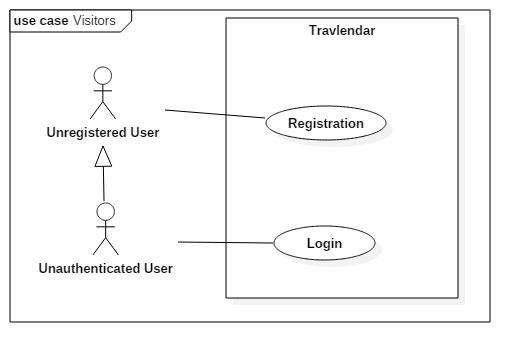
\includegraphics{Visitors.png}
	\subsubsection{User}
		\noindent\makebox[\textwidth]{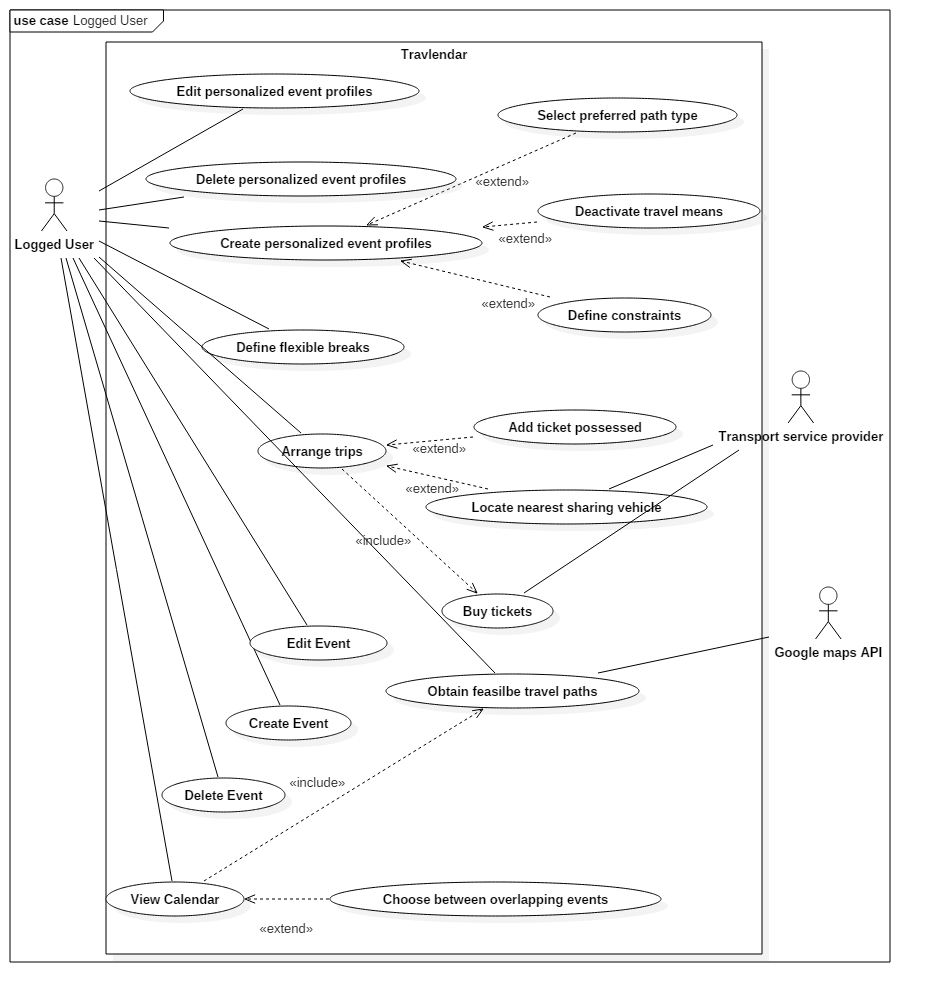
\includegraphics[width=\paperwidth,height=\paperheight,keepaspectratio]{LoggedUser.png}}